\documentclass[10pt,t,aspectratio=169]{beamer}
%\usetheme{Berkeley}
\usepackage{graphicx}
\usepackage{amsmath}
\usepackage[american]{circuitikz}

% Packages to plot functions
\usepackage{pgfplots}
\pgfplotsset{compat=newest}

\usepackage{multicol}
\usepackage{multirow}
\usepackage{textcomp} % to use \textmu
\usepackage[absolute,overlay]{textpos} % to place floating text boxes with \begin{textblock*}{width}(x,y)
\usepackage{tcolorbox}
\usepackage{colortbl} % allows coloring cells of a table with \cellcolor{blue!25}

\title{Clase 5}
\subtitle{Deformación de bandas}
\author{Dr.-Ing. Juan José Montero Rodríguez}
\subject{Elementos Activos}
\institute{Escuela de Ingeniería Electrónica}
\date{Semestre II-2023}
\titlegraphic{
\includegraphics[height=12mm]{figures/logoTEC.pdf}}


\begin{document}

\begin{frame}[t]
\titlepage
\end{frame}



\begin{frame}[t]
    \frametitle{Diagrama de Bandas en Equilibrio}

    \begin{columns}
    
        \begin{column}{0.5\textwidth}
        
            El diagrama de bandas de energía para silicio tipo n no degenerado, en equilibrio térmico y sin luz externa aplicada, se muestra en la figura.

            \vspace{3mm}
            \begin{itemize}
                \item $E_V$: banda de valencia
                \item $E_C$: banda de conducción
                \item $E_{vac}$: nivel de vacío
                \item $\chi$: afinidad electrónica
                \item $\phi$: función de trabajo
            \end{itemize}
            
        \end{column}
        
        \begin{column}{0.5\textwidth}
        
            \centering
            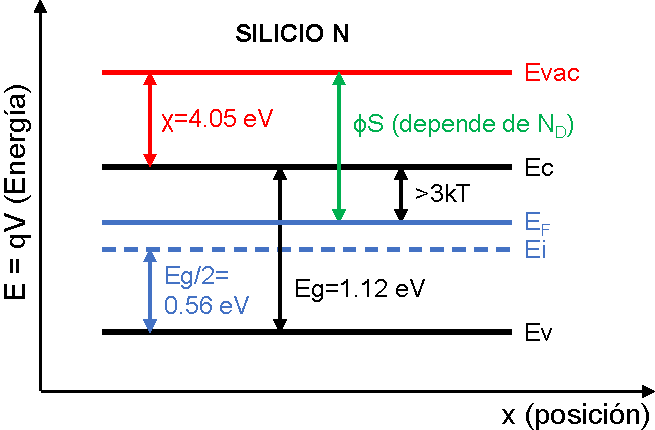
\includegraphics[width=\textwidth]{./figures/bandas-equilibrio.pdf}
            
        \end{column}
        
    \end{columns}
    
    \begin{itemize}
        \item Las bandas son planas indicando que la energía es la misma en cualquier posición del cristal.
        \item La energía está definida para un electrón.
        \item El eje vertical indica que la \textbf{energía aumenta}.
        \item El eje vertical indica que el \textbf{potencial disminuye}.
    \end{itemize}
\end{frame}


\begin{frame}[t]
    \frametitle{Doblamiento de Bandas}

    \begin{itemize}
        \item Los materiales estudiados hasta el momento se encuentran en estado de equilibrio térmico (sin tensión aplicada, temperatura constante, sin luz).
        \item El diagrama de bandas es plano indicando que E no varía con la posición.
        \item Cuando se asumen condiciones fuera de equilibrio térmico, existe \textbf{deformación de bandas} o \textbf{doblamiento de bandas}.
        \item Esto sucede en los siguientes escenarios:
        \begin{itemize}
            \item \textbf{Tensión aplicada} en una sección del material
            \item \textbf{Contacto} de dos materiales con distintos niveles de energía
            \begin{itemize}
                \item Dos metales (efecto Seebeck)
                \item Metal-semiconductor (contacto óhmico y contacto Schottky)
                \item Semiconductor-semiconductor (unión PN = diodo)
            \end{itemize}
        \end{itemize}
    \end{itemize}
\end{frame}


\begin{frame}[t]
    \frametitle{Doblamiento de Bandas con Potencial Aplicado}

    Cuando hay un campo eléctrico $\mathcal{E}$ en el semiconductor, el diagrama de bandas se deforma $\rightarrow$ bandas dependen de la posición $x$

    \begin{columns}
    
        \begin{column}{0.5\textwidth}
        
            \centering
            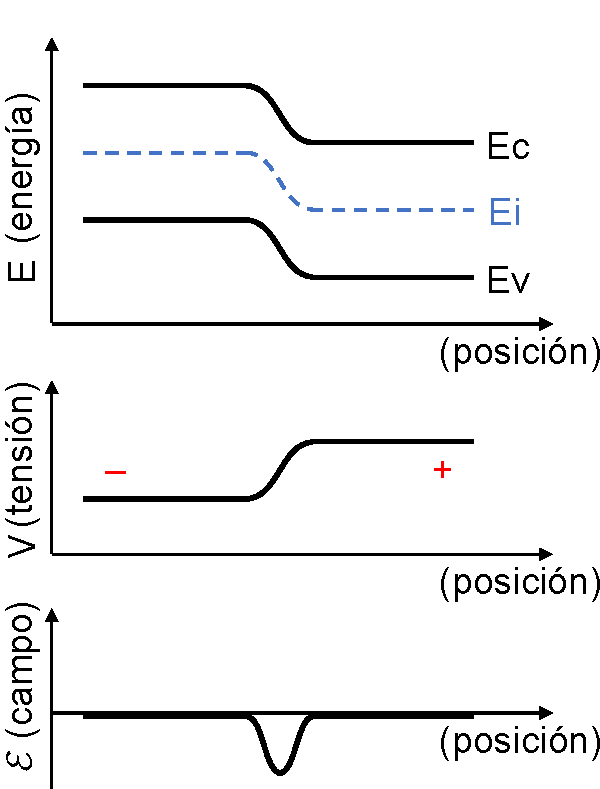
\includegraphics[width=4.5cm]{./figures/bandas-con-potencial.pdf}
            
        \end{column}
        
        \begin{column}{0.5\textwidth}
        
            La relación entre potencial y campo:
            %
            \[ E = qV \]
            %
            El potencial se calcula como:
            %
            \[ V = \dfrac{1}{q} (E_C - E_{ref}) \]
            %
            %Por lo tanto $V$ es un espejo de la banda de conducción $E_C$
            %
            El campo eléctrico $\mathcal{E}$ se define como:
            %
            \[ \mathcal{E} = \nabla{}V = \dfrac{dV}{dx} \]
            %
            %Por lo tanto $\mathcal{E}$ es la primera derivada de la banda de conducción $E_C$
            %
            \textbf{Recordatorio: la carga ``q'' es negativa.}
            
        \end{column}
        
    \end{columns}
    
\end{frame}


\begin{frame}[t]
    \frametitle{Doblamiento de Bandas en Contactos S-S}

    \begin{tcolorbox}
        \centering
        Al unir dos materiales distintos, los niveles de Fermi se alinean.
    \end{tcolorbox}

    \begin{columns}
    
        \begin{column}{0.5\textwidth}
        
            Considere el diagrama de bandas del silicio p y el silicio n por separado.

            \begin{itemize}
                \item Silicio 1: (tipo p: $\phi_{S1} = 4.72\ eV$)
                \item Silicio 2: (tipo n, $\phi_{S2} = 4.50\ eV$)
            \end{itemize}

            \vspace{2mm}
            Al unir los dos materiales, existe un \textbf{intercambio de portadores} que alinea los niveles de Fermi de ambos materiales

            \begin{itemize}
                \item Las bandas del Si p suben
                \item Las bandas del Si n bajan
            \end{itemize}
            
            \vspace{2mm}
            En estado de equilibrio, el nivel de Fermi es constante y totalmente horizontal.
            
        \end{column}
        
        \begin{column}{0.5\textwidth}
        
            \centering
            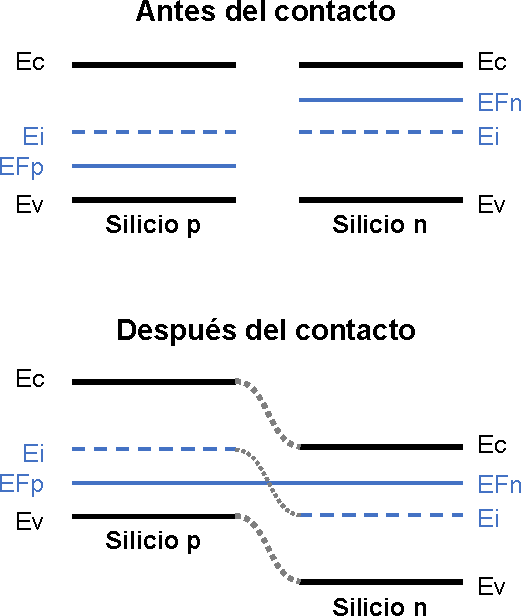
\includegraphics[height=5.5cm]{./figures/contacto-sin-sip.pdf}
            
        \end{column}
        
    \end{columns}

\end{frame}


\begin{frame}[t]
    \frametitle{Doblamiento de Bandas en Contactos M-S}

    \begin{tcolorbox}
        \centering
        Al unir dos materiales distintos, los niveles de Fermi se alinean.
    \end{tcolorbox}

    \begin{columns}
    
        \begin{column}{0.5\textwidth}
        
            Considere el diagrama de bandas de un metal y un semiconductor.

            \begin{itemize}
                \item Metal: Au (oro, $\phi_{M} = 5.1\ eV$)
                \item Silicio: (tipo n, $\phi_{S} = 4.50\ eV$)
            \end{itemize}

            \vspace{2mm}
            Al unir los dos materiales, existe un \textbf{intercambio de portadores} que alinea los niveles de Fermi de ambos materiales

            \begin{itemize}
                \item La función de trabajo de ambos materiales permanece constante.
            \end{itemize}
            
            \vspace{2mm}
            En estado de equilibrio, el nivel de Fermi es constante y totalmente horizontal.
            
        \end{column}
        
        \begin{column}{0.5\textwidth}
        
            \centering
            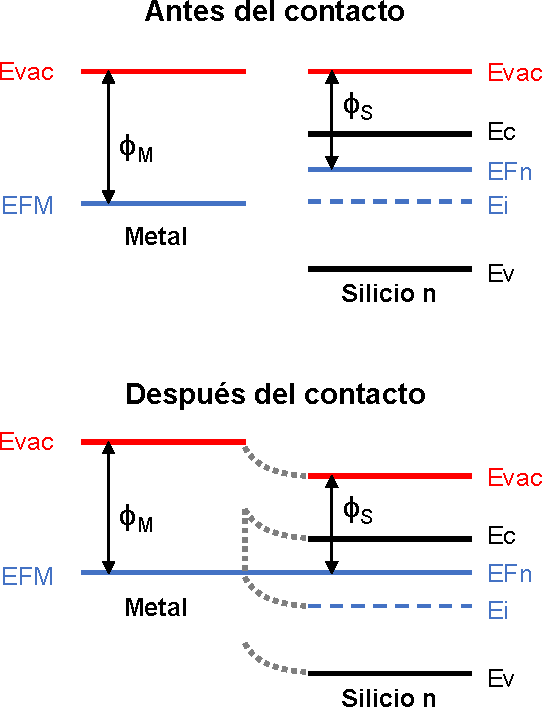
\includegraphics[height=5.5cm]{./figures/contacto-metal-silicio.pdf}
            
        \end{column}
        
    \end{columns}

\end{frame}


\begin{frame}[t]
    \frametitle{Doblamiento de Bandas en Contactos M-S}

    \begin{figure}[t]
        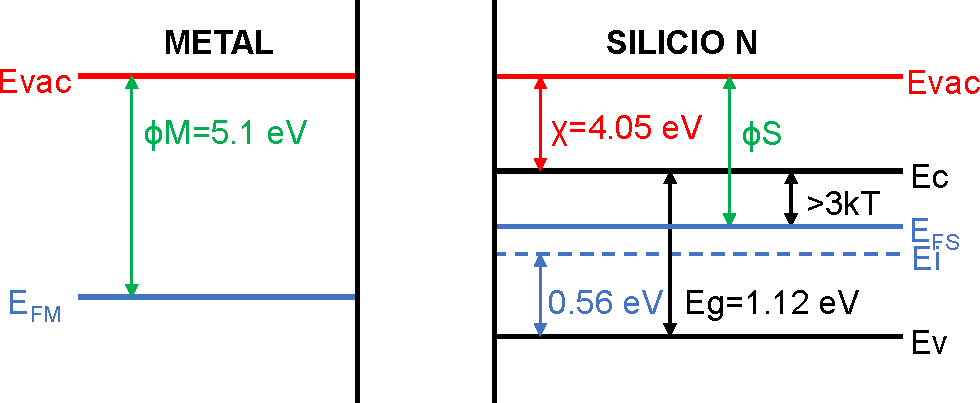
\includegraphics[scale=0.6]{./figures/contacto-MS-1.pdf}
    \end{figure}

    \begin{itemize}
        \item Un trozo de metal y un trozo de semiconductor se unen sin defectos.
        \item Los materiales antes del contacto están separados por una barrera.
    \end{itemize}
\end{frame}


\begin{frame}[t]
    \frametitle{Doblamiento de Bandas en Contactos M-S}

    \begin{figure}[t]
        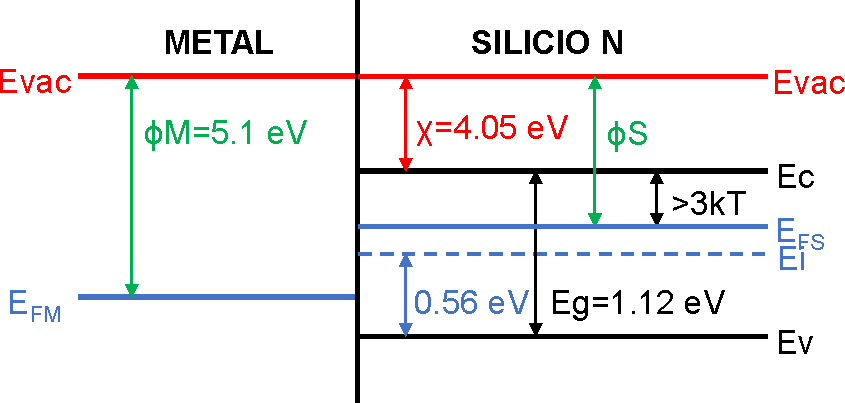
\includegraphics[scale=0.6]{./figures/contacto-MS-2.pdf}
    \end{figure}

    \begin{itemize}
        \item Los materiales entran en contacto directo, se asume que no hay defectos en la interfaz.
        \item El nivel de Fermi del semiconductor se debe alinear con el del metal.
    \end{itemize}
\end{frame}


\begin{frame}[t]
    \frametitle{Doblamiento de Bandas en Contactos M-S}

    \begin{figure}[t]
        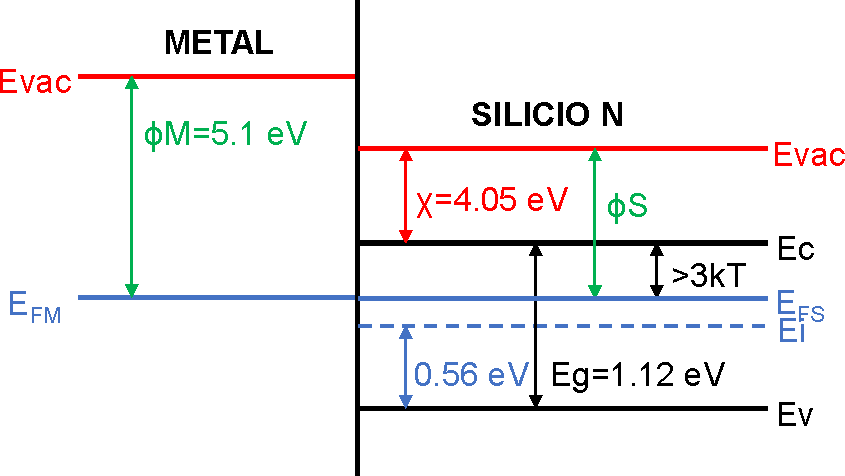
\includegraphics[scale=0.6]{./figures/contacto-MS-3.pdf}
    \end{figure}

    \begin{itemize}
        \item Las bandas del silicio se desplazan hacia abajo: los electrones del silicio tipo n ‘saltan’ hacia el metal, dejando una carga positiva en el semiconductor.
        \item El potencial positivo que queda en el semiconductor desplaza las bandas hacia abajo. Este potencial se denomina \textbf{potencial de contacto}.
    \end{itemize}
\end{frame}


\begin{frame}[t]
    \frametitle{Doblamiento de Bandas en Contactos M-S}

    \begin{figure}[t]
        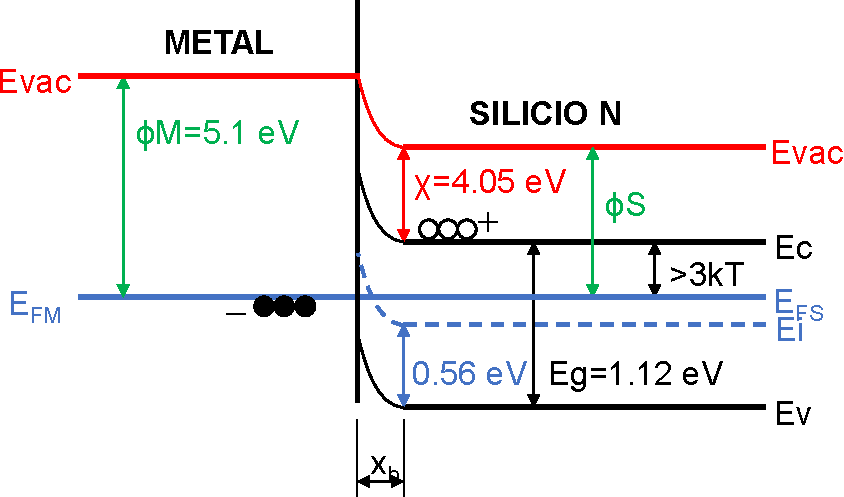
\includegraphics[scale=0.6]{./figures/contacto-MS-4.pdf}
    \end{figure}

    \begin{itemize}
        \item En el punto de contacto debe existir continuidad en las bandas. Por lo tanto, las bandas se curvan en una distancia $x_b$.
    \end{itemize}
\end{frame}


\begin{frame}[t]
    \frametitle{Doblamiento de Bandas en Contactos M-S}

    \begin{figure}[t]
        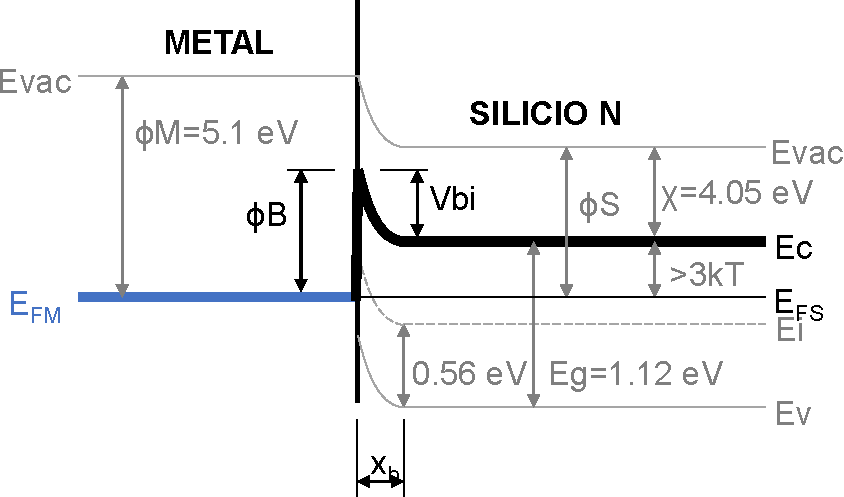
\includegraphics[scale=0.6]{./figures/contacto-MS-5.pdf}
    \end{figure}

    \begin{itemize}
        \item Analizando la forma que tiene la banda de conducción, se aprecia que ahora existe una \textbf{barrera de potencial} para los electrones a ambos lados.
        \item Los electrones \textbf{no pueden pasar} de izquierda a derecha, ni de derecha a izquierda, debido a que deben superar dos barreras de potencial.
    \end{itemize}
\end{frame}

\begin{frame}[t]
    \frametitle{Potencial y Campo Eléctrico en Contacto M-S}

    \begin{columns}
    
        \begin{column}{0.5\textwidth}
        
            \centering
            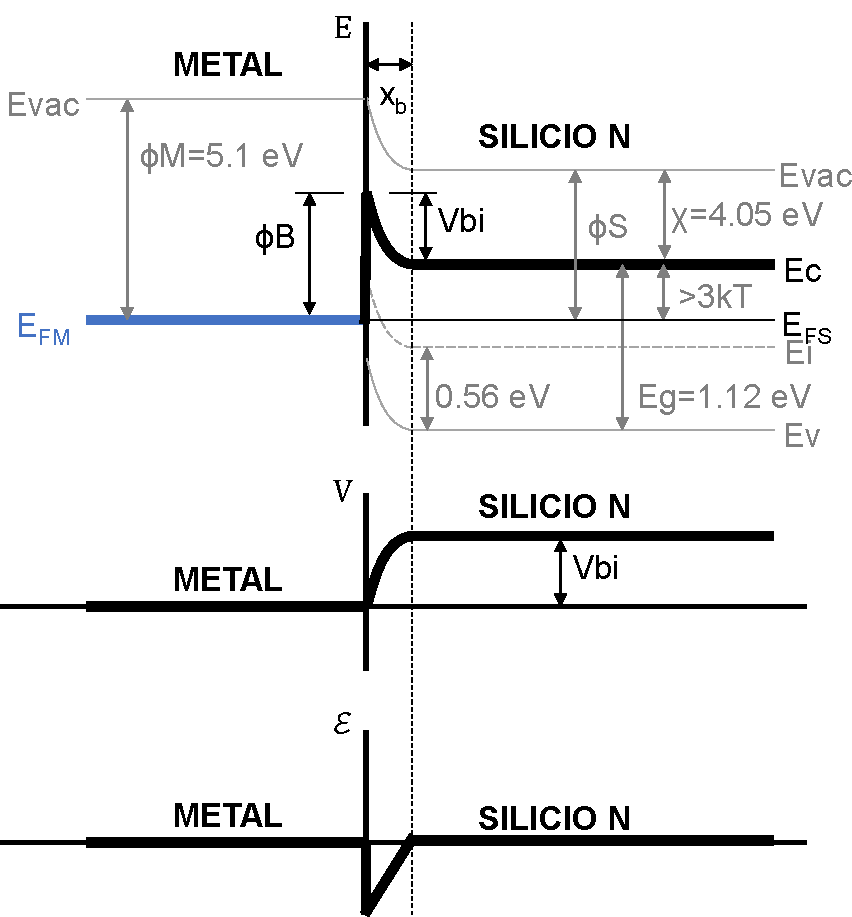
\includegraphics[height=7cm]{./figures/contacto-MS-6.pdf}
            
        \end{column}
        
        \begin{column}{0.5\textwidth}
        
            Si las bandas se curvan, es posible graficar el potencial y el campo eléctrico en función de la posición.

            \begin{itemize}
                \item La energía $E$ es función de la posición $x$.
                \item El potencial $V(x)$ es el opuesto de la banda de conducción.
                \[ V = \dfrac{1}{q}(E_C - E_{ref}) \]
                \item El campo eléctrico $\mathcal{E}(x)$ es la primera derivada de la banda de conducción.
                \[ \mathcal{E} = \nabla{}V \]
            \end{itemize}
            
        \end{column}
        
    \end{columns}
    
\end{frame}


\begin{frame}[t]
    \frametitle{Carga: Ecuación de Poisson}

    \begin{tcolorbox}
        \centering\textbf{Los electrones que `saltan' del semiconductor al metal dejan una carga eléctrica asociada: positiva en el semiconductor, negativa en el metal.}
    \end{tcolorbox}

    \begin{itemize}
        \item La carga eléctrica se relaciona con el campo eléctrico por medio de la Ecuación de Poisson:
    \end{itemize}
    %
    \begin{columns}
    
        \begin{column}{0.4\textwidth}
        
            \[ \dfrac{d\mathcal{E}}{dx} = \dfrac{\rho}{\epsilon_0 \epsilon_r} = \dfrac{q N_D}{\epsilon_0 \epsilon_r} \]
            
        \end{column}
        
        \begin{column}{0.6\textwidth}
        
            \begin{itemize}
                \item $\epsilon_0$: permitividad del vacío ($8.85\times{}10^{-14}\ F\cdot{}cm^{-1}$)
                \item $\epsilon_r$: permitividad relativa (Si: 11.7, Ge: 16.2)
                \item $\rho$: densidad de carga eléctrica [C/cm\textsuperscript{-3}]
            \end{itemize}
            
        \end{column}
        
    \end{columns}

    \vspace{2mm}
    \begin{itemize}
        \item Para el ejemplo estudiado en la diapositiva anterior, la densidad de carga:
    \end{itemize}

    \begin{columns}
    
        \begin{column}{0.5\textwidth}
        
            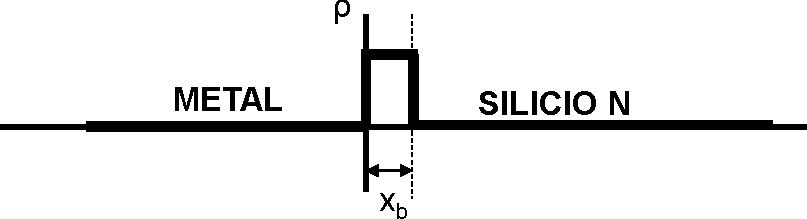
\includegraphics[width=\textwidth]{./figures/contacto-MS-7.pdf}
            
        \end{column}
        
        \begin{column}{0.5\textwidth}
        
            El ancho de la región $x_b$ al aplicar $V_A$:
            \[ x_b = \sqrt{\dfrac{2\epsilon_0\epsilon_r(V_{bi}-V_A)}{qN_D}} \]
            
        \end{column}
        
    \end{columns}
    
\end{frame}


\begin{frame}[t]
    \frametitle{Barrera Schottky y Potencial de Contacto}

    \begin{columns}
        \begin{column}{0.5\textwidth}
            \begin{itemize}
                \item La barrera Schottky $\phi_B$ se puede calcular (en eV) como:
            \end{itemize}
            %
            \[ \phi_B = \phi_M - \chi \]
            %
            \[ \phi_B = \dfrac{kT}{q}\ln{}\left(\dfrac{n_b}{n_i}\right) \]
            %
            \[ \phi_B = 60\ mV\ \log{}\left(\dfrac{n_b}{n_i}\right) \]
        \end{column}
        \begin{column}{0.5\textwidth}
            \begin{itemize}
                \item El potencial de contacto $V_{bi}$ se puede calcular (en V) como:
            \end{itemize}
            %
            \[ V_{bi} = \dfrac{1}{q}\left[ \phi_B - (E_C - E_F) \right] \]
            %
            Este potencial se define en ausencia de tensión aplicada.
        \end{column}
    \end{columns}

    \vspace{2mm}
    \centering
    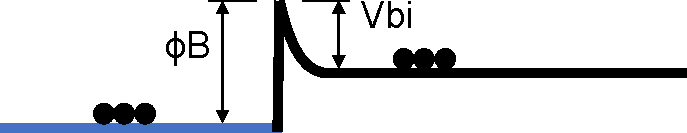
\includegraphics[width=7cm]{./figures/contacto-MS-8.pdf}

    \begin{itemize}
        \item Los electrones del metal NO pueden pasar al semiconductor porque existe una barrera $\phi_B$ que no se puede superar.
        \item Los electrones del semiconductor NO pueden pasar al metal porque existe una barrera $V_{bi}$ que no se puede superar.
    \end{itemize}
\end{frame}


\begin{frame}[t]
    \frametitle{Barrera Schottky y Potencial de Contacto con V Aplicada}

    \begin{itemize}
        \item Si se aplica una tensión positiva en el metal y negativa en el semiconductor con una magnitud igual a Vbi: los electrones pueden fluir de S$\rightarrow$M
        
        \centering
        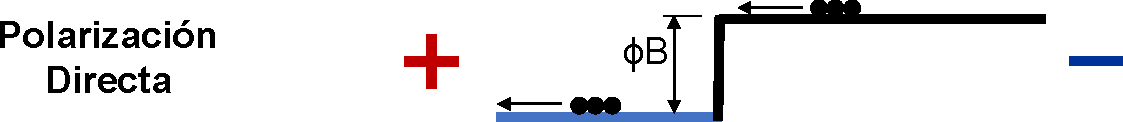
\includegraphics[width=11cm]{./figures/contacto-MS-9a.pdf}

        \flushleft
        \item Si la tensión aplicada excede Vbi, los electrones siguen fluyendo:

        \centering
        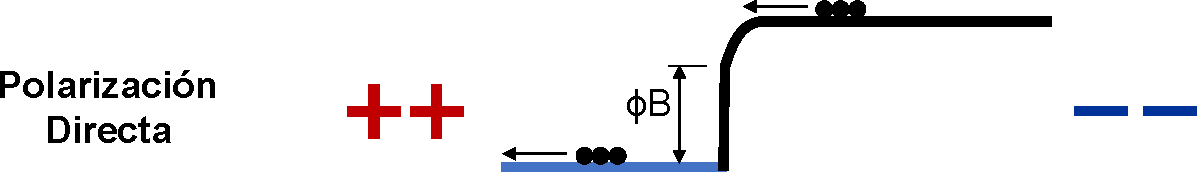
\includegraphics[width=11cm]{./figures/contacto-MS-9b.pdf}

        \flushleft
        \item Si se aplica una tensión positiva en el semiconductor y negativa en el metal la barrera Schottky permanece constante: electrones no fluyen M$\rightarrow$S

        \centering
        
\includegraphics[width=11cm]{./figures/contacto-MS-9c.pdf}
    \end{itemize}
\end{frame}


\begin{frame}[t]
    \frametitle{Diodo Schottky: Ánodo y Cátodo}

    \begin{itemize}
        \item El comportamiento que acabamos de describir demuestra que existe un flujo de corriente sólo en una dirección: contacto rectificante o diodo Schottky.
        \begin{itemize}
            \item El diodo Schottky tiene dos terminales: un ánodo y un cátodo
            \item La corriente técnica (cargas positivas) fluye de ánodo a cátodo
            \item Cátodo: terminal donde la corriente convencional sale del dispositivo
        \end{itemize}
    \end{itemize}

    \begin{columns}
        \begin{column}{0.5\textwidth}
            \centering
            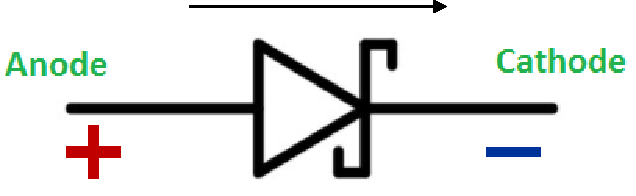
\includegraphics[width=0.6\textwidth]{./figures/diodo-schottky-1.pdf}
        \end{column}
        \begin{column}{0.5\textwidth}
            \centering
            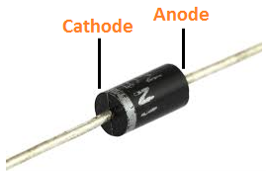
\includegraphics[width=0.6\textwidth]{./figures/diodo-schottky-2.png}
        \end{column}
    \end{columns}

    \begin{itemize}
        \item De acuerdo con las características del contacto estudiado, ¿cuál material forma el ánodo y cuál material forma el cátodo?
    \end{itemize}

    \begin{tcolorbox}
        \centering\textbf{Ánodo:} Metal | \textbf{Cátodo:} Semiconductor | Válido sólo para metal-silicio n con $\phi_M > \phi_S$
    \end{tcolorbox}
\end{frame}


\begin{frame}[t]
    \frametitle{Ejemplo: Hoja de Datos 1N5711}
    
    Diodo Schottky de baja potencia

    \begin{itemize}
        \item Observe la corriente cuando se aplica una tensión de directa $V_F = 0.6\ V$
        \item Compare con la corriente para una tensión de reversa $V_R = 0.6\ V$
    \end{itemize}

    \centering
    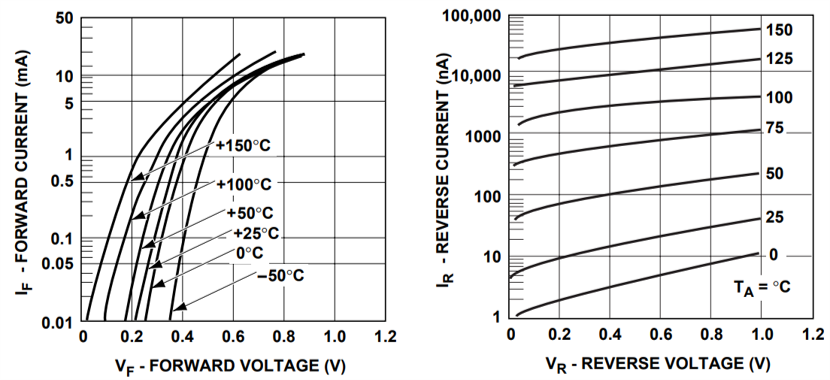
\includegraphics[width=12cm]{./figures/diodo-schottky-3.png}
\end{frame}


\begin{frame}[t]
    \frametitle{Ejemplo: Contacto Metal con Silicio p}

    Se tiene un contacto oro-silicio p a temperatura ambiente, donde existe una concentración de átomos dopantes igual a $2.1\times{}10^{16}\ cm^{-3}$.

    \begin{enumerate}
        \item Calcule la posición del nivel de Fermi del silicio.
        \item Calcule la función de trabajo del silicio.
        \item Dibuje el diagrama de bandas de energía antes del contacto.
        \item Determine si las bandas se mueven hacia arriba o hacia abajo.
        \item Dibuje el diagrama de bandas de energía después del contacto.
        \item Indique si existe una barrera de potencial para los electrones del metal.
        \item Indique si existe una barrera de potencial para los huecos del Si.
        \item Calcule el valor que tienen las barreras de potencial, si hubiera.
        \item Dibuje por inspección la forma que tiene el potencial V.
        \item Dibuje por inspección la forma que tiene el campo eléctrico $\mathcal{E}$.
        \item Dibuje por inspección la forma que tiene la densidad de carga $\rho$.
    \end{enumerate}
\end{frame}


\begin{frame}{Lecturas recomendadas}
    
\end{frame}

\end{document}
